\documentclass{report}

\usepackage[linesnumbered,ruled,vlined]{algorithm2e}
\usepackage{multirow}
\usepackage{rotating}
\usepackage{pdfpages}
\usepackage{graphicx}

\usepackage{tikz}
\usetikzlibrary{matrix}
\usepackage{preview}
\PreviewEnvironment{tikzpicture}

\author{GUELFEN Abdelheq}
\title{Devoir de AAC}

\begin{document}
\includepdf[pages=-]{coverPage.pdf}
\clearpage

\tableofcontents
\newpage

\section{Introduction}
Les graphes, essentiels pour modéliser des situations réelles, trouvent leur application dans divers domaines tels que les réseaux routiers, les systèmes informatiques, ou encore la planification de projets. Dans ce projet, nous nous concentrons sur la manière de stocker ces graphes dans un ordinateur et sur les opérations courantes associées. Deux méthodes principales, la matrice d'adjacence et la liste d'adjacence, seront explorées pour comprendre comment elles influent sur la complexité, c'est-à-dire l'espace mémoire requis et le temps d'exécution des opérations. Cette exploration vise à fournir des insights pratiques pour utiliser efficacement les graphes dans la résolution de problèmes concrets.

\section{Objectifs de travail}
Rappels sur la représentation de graphes en mémoire (différentes représentations)
Opérations sur les graphes avec calcul de complexité
Evaluation et comparaison de complexités théoriques et expérimentales

\section{Partie I}
On a établir les principales définition de la structure de graphe

\begin{itemize}
    \item{\textbf{Graphe}: est un ensemble de relations entre un ou plusieurs objets.}
    \item{\textbf{Graphe orienté}: est un graphe dans lequel chaque sommet a une direction spécifique.}
    \item{\textbf{Graphe non orienté}: est un graphe dans lequel les sommet n'ont pas de direction spécifique.}
    \item{\textbf{arête}: est une relation entre deux sommets dans un graphe non orienté.}
    \item{\textbf{arc}: est une relation entre deux nœuds dans un graphe orienté.}
    \item{\textbf{cycle}: est une séquence d'arêtes qui forme une boucle fermée dans un graphe.}
    \item{\textbf{circuit}: est un cycle qui parcourt tous les sommets d'un graphe eulérien.}
    \item{\textbf{graphe pondéré}: est un graphe dans lequel chaque arête a une valeur associée, généralement numérique, appelée poids.}
    \item{\textbf{degré d’un nœud}: est le nombre d'arêtes incidentes à ce nœud.}
    \item{\textbf{arc entrant}: est une arête qui se termine au nœud sans en sortir.}
    \item{\textbf{arc sortant}: est une arête qui part du nœud sans y entrer.}
    \item{\textbf{Graphe simple}: est un graphe sans boucles (arêtes reliant un nœud à lui-même) ni arêtes multiples entre les mêmes paires de nœuds.}
    \item{\textbf{multi-graphe}: Un multi-graphe permet d'avoir plusieurs arêtes entre les mêmes paires de nœuds.}
    \item{\textbf{graphe eulérien}: est un graphe qui contient un circuit eulérien, passant par chaque arête exactement une fois.}
    \item{\textbf{arbre}: Un arbre est un graphe orienté sans cycle, et muni d’une racine.}
    \item{\textbf{Densité d’un graphe}: La densité d'un graphe est le rapport entre le nombre d'arêtes présentes et le nombre d'arêtes potentielles dans un graphe complet.}
    \item{\textbf{graphe connexe}: Un graphe connexe est un graphe dans lequel il existe un chemin entre chaque paire de nœuds.}
    \item{\textbf{composante connexe}: Une composante connexe est un sous-graphe maximal dans un graphe non orienté connexe.}
    \item{\textbf{profondeur}:  La profondeur d'un nœud dans un graphe est la longueur du plus court chemin depuis un nœud racine jusqu'à ce nœud}
    \item{\textbf{graphe complet}: Un graphe complet est un type particulier de graphe non orienté dans lequel il existe une arête entre chaque paire distincte de nœuds.}
\end{itemize}

\section{Partie II}
Les représentations d’un graphe en mémoire

\begin{itemize}
  \item{\textbf{La definition de matrice d’adjacence: } La matrice d'adjacence est une représentation tabulaire d'un graphe où chaque élément M[i][j] indique s'il existe une arête entre les sommets i et j.La matrice utlise utilise (0 ou 1) pour représenter l'absence ou la présence d'une arête.}
  \item{\textbf{La definition de liste d’adjacence: } La liste d'adjacence est une représentation basée sur des tableaux ou des listes où chaque sommet du graphe est associé à une liste de ses voisins (les sommets auxquels il est directement connecté).}
\end{itemize}

\subsection{Graphe 1}
\begin{minipage}{0.5\textwidth}
    \subsubsection*{La matrice d'adjacence}
    \begin{tabular}{|lr|l|l|l|l|l|l|l|l|l|} \cline{3-8}
    \multicolumn{1}{l}{} & & a & b & c & d & e & f \\ \hline
    %                           A   B   C   D   E   F
    & \multicolumn{1}{|r|}{a} & 0 & 1 & 0 & 0 & 0 & 0 \\ \cline{2-8}
    & \multicolumn{1}{|r|}{b} & 0 & 0 & 1 & 0 & 0 & 0 \\ \cline{2-8}
    & \multicolumn{1}{|r|}{c} & 1 & 0 & 0 & 1 & 1 & 0 \\ \cline{2-8}
    & \multicolumn{1}{|r|}{d} & 0 & 0 & 0 & 0 & 1 & 0 \\ \cline{2-8}
    & \multicolumn{1}{|r|}{e} & 0 & 0 & 0 & 1 & 0 & 1 \\ \cline{2-8}
    & \multicolumn{1}{|r|}{f} & 0 & 1 & 0 & 0 & 0 & 0 \\ \hline
    \end{tabular}
\end{minipage}
\begin{minipage}{0.5\textwidth}
    \subsubsection*{La liste d'adjacence}
    \begin{tikzpicture}
        \matrix (M) [matrix of nodes,
        column sep=1pt,
        row sep=5pt,
        nodes={draw,fill=gray!13,minimum width=.8cm,outer sep=0pt,minimum
        height=.7cm,anchor=center},
        column 1/.style={minimum height=.8cm}]{
            \mbox{}&[5mm]b&/ \mbox{}&[3mm] & &[2mm] & & & \\
            \mbox{}&c&/ & & & & & & \\
            \mbox{}&a& \mbox{}&d& \mbox{}&e&/ & & \\
            \mbox{}&e&/ \mbox{}& & & & & & \\
            \mbox{}&d& \mbox{}&f&/ & & & & \\
            \mbox{}&b&/ \mbox{}& & & & & & \\
        };

        \foreach \i/\label in {1/a, 2/b, 3/c, 4/d, 5/e, 6/f}{
            \path (M-\i-1) [late options={label=left:\label}];
            \draw[->] (M-\i-1.center)--(M-\i-2.west);
        }

        % C node
        \draw[->] (M-3-3.center)--(M-3-4.west);
        \draw[->] (M-3-5.center)--(M-3-6.west);

        % E node
        \draw[->] (M-5-3.center)--(M-5-4.west);
    \end{tikzpicture}
\end{minipage}

\subsection{Graphe 2}
\begin{minipage}{0.5\textwidth}
    \subsubsection*{La matrice d'adjacence}
    \begin{tabular}{|lr|l|l|l|l|} \cline{3-6}
    \multicolumn{1}{l}{} & & 1 & 2 & 3 & 4 \\ \hline
    %                           1   2   3   4
    & \multicolumn{1}{|r|}{1} & 0 & 0 & 0 & 1 \\ \cline{2-6}
    & \multicolumn{1}{|r|}{2} & 1 & 1 & 0 & 0 \\ \cline{2-6}
    & \multicolumn{1}{|r|}{3} & 1 & 1 & 1 & 1 \\ \cline{2-6}
    & \multicolumn{1}{|r|}{4} & 1 & 1 & 1 & 0 \\ \hline
    \end{tabular}
\end{minipage}
\begin{minipage}{0.5\textwidth}
    \subsubsection*{La liste d'adjacence}
    \begin{tikzpicture}
        \matrix (M) [matrix of nodes,
        column sep=1pt,
        row sep=5pt,
        nodes={draw,fill=gray!13,minimum width=.8cm,outer sep=0pt,minimum
        height=.7cm,anchor=center},
        column 1/.style={minimum height=.8cm}]{
            \mbox{}&[5mm]4&/ \mbox{}&[3mm] & &[2mm] & &[2mm] & \\
            \mbox{}&1& \mbox{}&2&/ & & & & \\
            \mbox{}&1& \mbox{}&2& \mbox{}&3& \mbox{}&4&/ \\
            \mbox{}&1& \mbox{}&2& \mbox{}&3&/ & & \\
        };

        \foreach \i/\label in {1, 2, 3, 4}{
            \path (M-\i-1) [late options={label=left:\label}];
            \draw[->] (M-\i-1.center)--(M-\i-2.west);
        }

        % 2 node
        \draw[->] (M-2-3.center)--(M-2-4.west);

        % 3 node
        \draw[->] (M-3-3.center)--(M-3-4.west);
        \draw[->] (M-3-5.center)--(M-3-6.west);
        \draw[->] (M-3-7.center)--(M-3-8.west);

        % 4 node
        \draw[->] (M-4-3.center)--(M-4-4.west);
        \draw[->] (M-4-5.center)--(M-4-6.west);
    \end{tikzpicture}
\end{minipage}

\subsection{Graphe 3}
\begin{minipage}{0.5\textwidth}
    \subsubsection*{La matrice d'adjacence}
    \begin{tabular}{|lr|l|l|l|l|l|l|l|l|l|} \cline{3-8}
    \multicolumn{1}{l}{} & & a & b & c & d & e & f \\ \hline
    %                           A   B   C   D   E   F
    & \multicolumn{1}{|r|}{a} & 0 & 1 & 0 & 0 & 0 & 1 \\ \cline{2-8}
    & \multicolumn{1}{|r|}{b} & 1 & 0 & 1 & 0 & 0 & 0 \\ \cline{2-8}
    & \multicolumn{1}{|r|}{c} & 0 & 1 & 0 & 1 & 0 & 0 \\ \cline{2-8}
    & \multicolumn{1}{|r|}{d} & 0 & 0 & 1 & 0 & 1 & 0 \\ \cline{2-8}
    & \multicolumn{1}{|r|}{e} & 0 & 0 & 0 & 1 & 0 & 1 \\ \cline{2-8}
    & \multicolumn{1}{|r|}{f} & 1 & 0 & 0 & 0 & 1 & 0 \\ \hline
    \end{tabular}
\end{minipage}
\begin{minipage}{0.5\textwidth}
    \subsubsection*{La liste d'adjacence}
    \begin{tikzpicture}
        \matrix (M) [matrix of nodes,
        column sep=1pt,
        row sep=5pt,
        nodes={draw,fill=gray!13,minimum width=.8cm,outer sep=0pt,minimum
        height=.7cm,anchor=center},
        column 1/.style={minimum height=.8cm}]{
            \mbox{}&[5mm]b& \mbox{}&[3mm]f&/ &[2mm] & & & \\
            \mbox{}&a& \mbox{}&c&/ & & & & \\
            \mbox{}&b& \mbox{}&d&/ & & & & \\
            \mbox{}&c& \mbox{}&e&/ & & & & \\
            \mbox{}&d& \mbox{}&f&/ & & & & \\
            \mbox{}&a& \mbox{}&e&/ & & & & \\
        };

        \foreach \i/\label in {1/a, 2/b, 3/c, 4/d, 5/e, 6/f}{
            \path (M-\i-1) [late options={label=left:\label}];
            \draw[->] (M-\i-1.center)--(M-\i-2.west);
            \draw[->] (M-\i-3.center)--(M-\i-4.west);
        }
    \end{tikzpicture}
\end{minipage}

\newpage
\section{Partie III}

\subsection{Construction d'un graphe}
\subsubsection{utilisant la matrice d'adjacence}
La complexite de cet algorithme est:\(O(n^{2})\)\\
on a deux boucle qui repete \(N\) fois

\begin{algorithm}
\KwData{M: matrice/entier}
\KwData{N: taille de graph/entier}
\For{i de 0 a N}{
  \For{j de 0 a N}{
    M[i][j] = 0
  }
}
\For{arc in arces}{
  M[arc[0]][arc[1]] = 1
}
\caption{}
\end{algorithm}

\subsubsection{utilisant la liste d'adjacence}

La complexite de cet algorithme est:\(O(n)\)\\
on a un seul boucle qui repete \(N\) fois
\begin{algorithm}
\KwData{T: tablaux/entier}
\KwData{N: taille de graph/entier}
\For{i de 0 a N}{
  T[i] = 0
}
\For{arc in arces}{
  M[arc[0]] = arc[1]
}
\caption{}
\end{algorithm}
\newpage
\subsection{Affichage de graphe}

\subsubsection{utilisant la matrice d'adjacence}
La complexite de cet algorithme est:\(O(n^{2})\)\\
on a deux boucle qui repete \(N\) fois
\begin{algorithm}
\KwData{M: matrice/entier}
\For{i de 0 a N}{
  \For{j de 0 a N}{
    printf(M[i][j])
  }
}
\caption{}
\end{algorithm}

\subsubsection{utilisant la liste d'adjacence}
La complexite de cet algorithme est:\(O(n*m)\)\\
on a deux boucle qui repete \(N\) et \(M\) fois respectivement
\begin{algorithm}
\KwData{T: tablaux/entier}
\KwData{M: taille de tablaux/entier}
\For{i de 0 a N}{
  printf(i)

  \For{j de 0 a M}{
    printf(T[i][j])
  }
}
\caption{}
\end{algorithm}

\subsection{Calcule de densité}

\subsubsection{utilisant la matrice d'adjacence}
\begin{algorithm}
\KwData{M: matrice/entier}
m = 0

n = 0

\For{i de 0 a N}{
  \For{j de 0 a N}{
    \If{M[i][j] == 1}{
      m = m + 1
    }
  }
}
\Return (2 * m) / (n * (n - 1))
\caption{}
\end{algorithm}
La complexite de cet algorithme est:\(O(n^{2})\)on a deux boucle qui repete \(N\) fois

\subsubsection{utilisant la liste d'adjacence}
La complexite de cet algorithme est:\(O(n*m)\)\\
on a deux boucle qui repete \(N\) et \(M\) fois respectivement
\begin{algorithm}
\KwData{M: matrice/entier}
m = 0

n = 0

\For{i de 0 a N}{
  n = n + 1

  \For{j de 0 a M}{
    m = m + 1
  }
}
\Return (2 * m) / (n * (n - 1))
\caption{}
\end{algorithm}

\subsection{Calcule de degre}
\subsubsection{utilisant la matrice d'adjacence}
La complexite de cet algorithme est:\(O(n^{2})\)\\
on a deux boucle qui repete \(N\) fois
\begin{algorithm}
\KwData{M: matrice/entier}
m = 0

n = 0

\For{i de 0 a N}{
  \For{j de 0 a N}{
    \If{M[i][j] == 1}{
      m = m + 1
    }
  }
}
\Return m
\caption{}
\end{algorithm}

\subsubsection{utilisant la liste d'adjacence}
La complexite de cet algorithme est:\(O(n)\)\\
on un seul boucle qui repete \(N\) fois
\begin{algorithm}
\KwData{M: matrice/entier}
m = 0

\For{i de 0 a N}{
  m = m + 1
}
\Return m
\caption{}
\end{algorithm}

\subsection{Verification de graphe complet}
\subsubsection{utilisant la matrice d'adjacence}
La complexite de cet algorithme est:\(O(n^{2})\)\\
on a deux boucle qui repete \(N\) fois
\begin{algorithm}
\KwData{M: matrice/entier}
m = 0

n = 0

\For{i de 0 a N}{
  \For{j de 0 a N}{
    \If{M[i][j] == 1}{
      m = m + 1
    }
  }
}
\Return m == n * (n - 1) / 2
\caption{}
\end{algorithm}

\subsubsection{utilisant la liste d'adjacence}
La complexite de cet algorithme est:\(O(n*m)\)\\
on a deux boucle qui repete \(N\) et \(M\) fois respectivement
\begin{algorithm}
\KwData{M: matrice/entier}
m = 0

n = 0

\For{i de 0 a N}{
  n = n + 1

  \For{j de 0 a M}{
    m = m + 1
  }
}
\Return m == n * (n - 1) / 2
\caption{}
\end{algorithm}

\subsection{Recherche d'un noeud dans le graphe}
\subsubsection{utilisant la matrice d'adjacence}
La complexite de cet algorithme est:\(O(n)\)\\
la complexite est paraport la taille de noeud
\begin{algorithm}
\KwData{M: matrice/entier}
T = []

\For{i de 0 a M[node]}{
  \If{M[node][i] == 1}{
    T[I] = 1
  }
}
\Return T
\caption{}
\end{algorithm}

\subsubsection{utilisant la liste d'adjacence}
La complexite de cet algorithme est:\(O(1)\)\\
c'est un algorithme constante
\begin{algorithm}
\KwData{G: graphe/entier}
\Return G[node]
\caption{}
\end{algorithm}

\subsection{Recherche de tous les chemins}
La complexite de cet algorithme est:\(O(n^{2})\)\\
On a un boucle avec une appelle recursive
\begin{algorithm}
\KwData{M: matrice/entier}
file = File()

visited = []

enfilier(file, node)

visited[0] = node

\While{non vide(file)}{
  currentnode = defilier(file)

  \For{neighbor in fils(currentnode)}{
    \If {neighbor not in visited}{
      dfs(neighbor)
    }
  }
}
\caption{}
\end{algorithm}
\newpage

\subsection{Recherche le chemin le plus court}
La complexite de cet algorithme est le meme de complexite de \(dfs()\)
\begin{algorithm}
\KwData{M: matrice/entier}
paths = dfs()

\Return min(paths)
\caption{}
\end{algorithm}


\section{Evaluation expérimentale}
On a effectué plusieurs tests avec des graphe de taille 10, 20, 50, et on a trouver ces resultats\\

\begin{tabular}{|c|c|c|c|c|}
    \hline
    Taille n & Construction(Tps) & Affichage(Tps) & Densité(Tps) & Dergee(Tps) \\
    \hline
    10 & 2.3e-05 & 2.36e-05 & 1.3e-05 & 9.05e-06 \\
    \hline
    20 & 2.6e-05 & 2.6e-05 & 1.4e-05 & 5.7e-06 \\
    \hline
    50 & 4.5e-05 & 4.5e-05 & 1.2e-05 & 6.9e-06\\
    \hline
\end{tabular}
\\
\\
\\
\\
\begin{tabular}{|c|c|c|c|c|}
    \hline
    Taille n & Graphe est complet(Tps) & Recherche(Tps) & Tous chemins(Tps) & petite chemin \\
    \hline
    10 & 1.7e-05 & 4.5e-06 & 6.6e-05 & 1.9e-05\\
    \hline
    20 & 1.4e-05 & 4.5e-06 & 4.05e-05 & 4.05e-05 \\
    \hline
    50 & 1.4e-05 & 4.7e-06 & 0.002 & 0.002\\
    \hline
\end{tabular}
\newpage

\section{Conclusion}
En résumé :\\
\textbf{Complexité spatiale:}
Matrice d'adjacence :\(O(n^{2})\) inefficace pour les grands graphes.
Liste d'adjacence : Espace proportionnel aux arêtes et sommets, plus efficace pour les graphes épars.\\

\textbf{Complexité temporelle:}
Matrice d'adjacence : Accès constant \(O(1)\), itération \(O(n^{2})\).
Liste d'adjacence : Performances temporelles généralement meilleures pour les graphes épars.\\

\textbf{Taille et densité:}
Matrice d'adjacence: Plus grande pour les graphes denses.
Liste d'adjacence : Plus performante pour les graphes épars.\\

En conclusion, la matrice d'adjacence offre un accès constant, mais son espace peut être inefficace pour les graphes épars. La liste d'adjacence est plus efficace pour ces graphes, offrant une meilleure performance pour de nombreuses opérations. Le choix dépend du cas d'utilisation, de la densité du graphe et des opérations envisagées.

\clearpage
\section{Annexe}
Quelque example d'afichage de graphes apres executer le source code
\begin{figure}[ht]
    \centering
    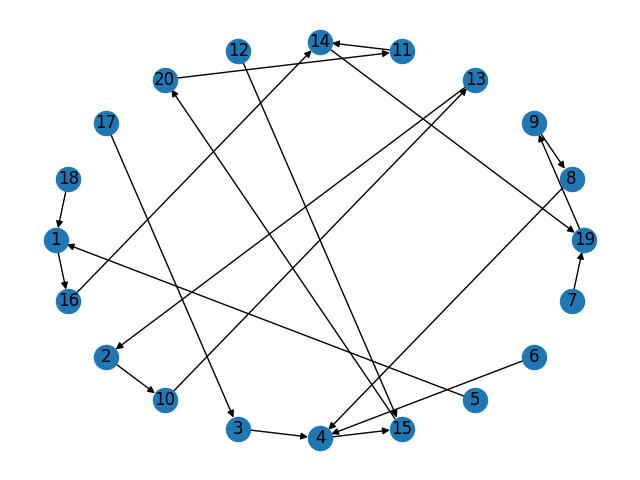
\includegraphics[width=0.5\textwidth]{./graph20.png}
    \caption{Une affichage de graphe de taille 10}
\end{figure}

\begin{figure}[ht]
    \centering
    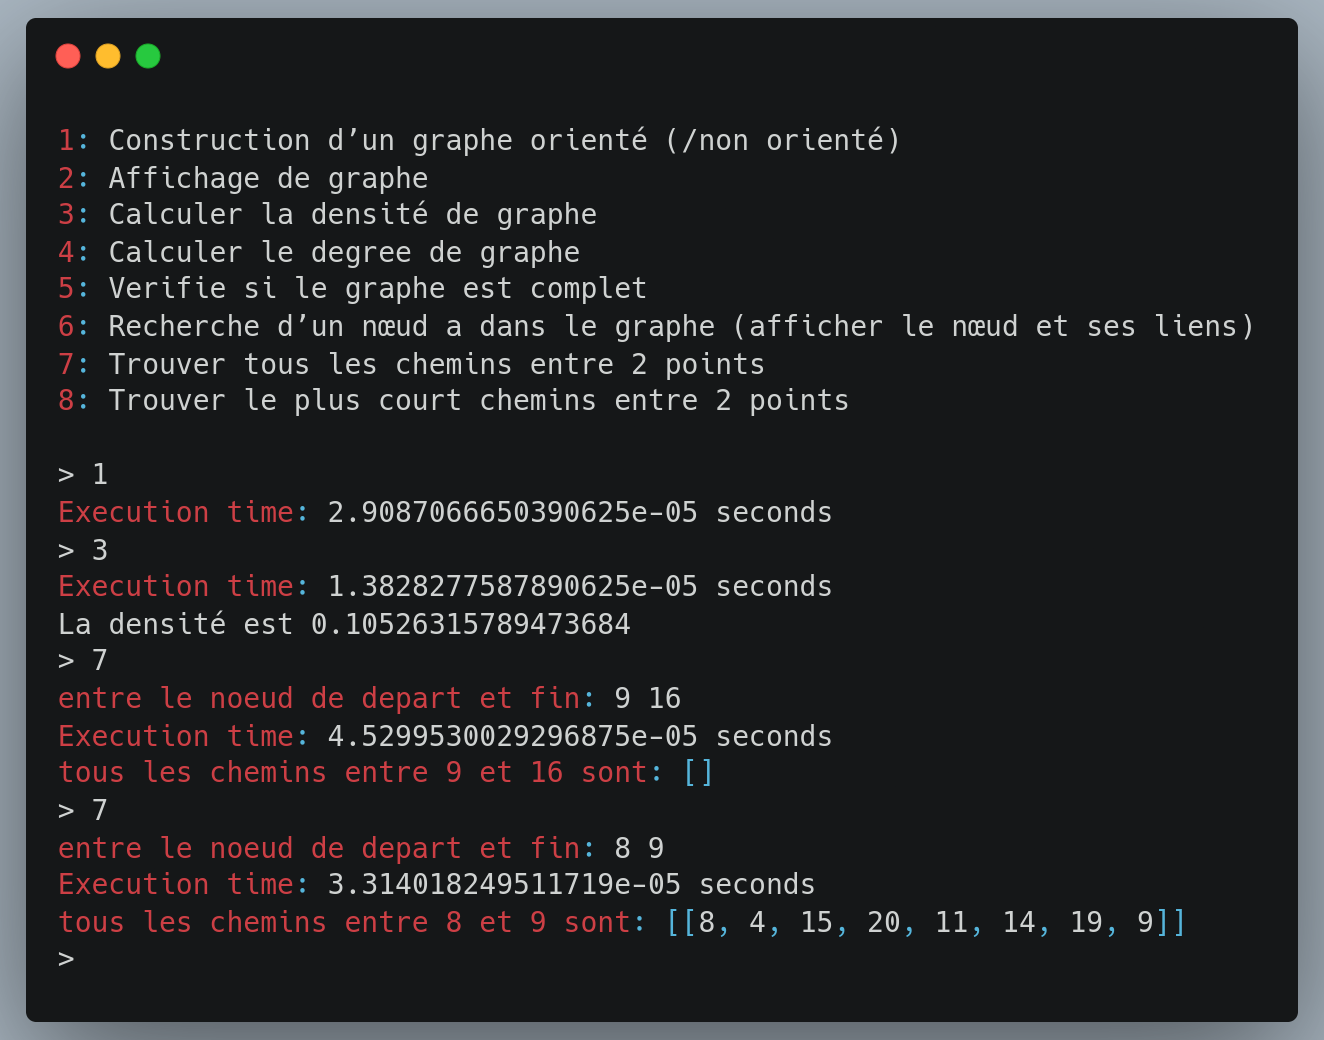
\includegraphics[width=0.8\textwidth]{./code.png}
    \caption{Capture d'ecran illustrant l'execution de quelque fonctions}
\end{figure}
\end{document}
